
\documentclass{article}
%%%%%%%%%%%%%%%%%%%%%%%%%%%%%%%%%%%%%%%%%%%%%%%%%%%%%%%%%%%%%%%%%%%%%%%%%%%%%%%%%%%%%%%%%%%%%%%%%%%%%%%%%%%%%%%%%%%%%%%%%%%%%%%%%%%%%%%%%%%%%%%%%%%%%%%%%%%%%%%%%%%%%%%%%%%%%%%%%%%%%%%%%%%%%%%%%%%%%%%%%%%%%%%%%%%%%%%%%%%%%%%%%%%%%%%%%%%%%%%%%%%%%%%%%%%%
%TCIDATA{OutputFilter=LATEX.DLL}
%TCIDATA{Version=5.50.0.2953}
%TCIDATA{<META NAME="SaveForMode" CONTENT="1">}
%TCIDATA{BibliographyScheme=Manual}
%TCIDATA{Created=Monday, March 12, 2012 12:19:48}
%TCIDATA{LastRevised=Monday, March 12, 2012 12:40:46}
%TCIDATA{<META NAME="GraphicsSave" CONTENT="32">}
%TCIDATA{<META NAME="DocumentShell" CONTENT="Standard LaTeX\Blank - Standard LaTeX Article">}
%TCIDATA{CSTFile=40 LaTeX article.cst}
\usepackage[pdftex]{graphicx}
\DeclareGraphicsExtensions{.pdf,.png,.jpg}
\newtheorem{theorem}{Theorem}
\newtheorem{acknowledgement}[theorem]{Acknowledgement}
\newtheorem{algorithm}[theorem]{Algorithm}
\newtheorem{axiom}[theorem]{Axiom}
\newtheorem{case}[theorem]{Case}
\newtheorem{claim}[theorem]{Claim}
\newtheorem{conclusion}[theorem]{Conclusion}
\newtheorem{condition}[theorem]{Condition}
\newtheorem{conjecture}[theorem]{Conjecture}
\newtheorem{corollary}[theorem]{Corollary}
\newtheorem{criterion}[theorem]{Criterion}
\newtheorem{definition}[theorem]{Definition}
\newtheorem{example}[theorem]{Example}
\newtheorem{exercise}[theorem]{Exercise}
\newtheorem{lemma}[theorem]{Lemma}
\newtheorem{notation}[theorem]{Notation}
\newtheorem{problem}[theorem]{Problem}
\newtheorem{proposition}[theorem]{Proposition}
\newtheorem{remark}[theorem]{Remark}
\newtheorem{solution}[theorem]{Solution}
\graphicspath{{D:/Dropbox/Private/FP/Gruppe34/FellesDoc/Ktn/}}
\newtheorem{summary}[theorem]{Summary}
\newenvironment{proof}[1][Proof]{\noindent\textbf{#1.} }{\ \rule{0.5em}{0.5em}}
\input{tcilatex}
\begin{document}


\part{The Design}

\section{Connection}

TCP employs a three way handshake to create a connection between two hosts.
This functionality can be realized by implementing the \texttt{connect()}
and \texttt{accept()} methods mentioned in the connection interface. The 
\texttt{connect()} method will handle the client side of the handshake,
while \texttt{accept()} will handle the server side.

The TCP client starts in the closed state. A new TCP is initiated by sending
a packet with the \texttt{SYN} bit set to 1, and its randomly chosen
internal sequence number. After the \texttt{SYN} segement is sent, the
client enters the \texttt{\texttt{SYN}\_SENT} state, waiting for the
corresponding \texttt{\texttt{SYN}\_ACK} from the server.

The server will respond to the \texttt{SYN} packet by sending a \texttt{%
\texttt{SYN}\_ACK} packet, with the \texttt{SYN} bit set to 1, its internal
sequence number, and the \texttt{ACK} field set to the next expected
sequence number.

When the client has received the \texttt{\texttt{SYN}\_ACK} packet, it
enters the \texttt{ESTABLISHED} state, and sends an \texttt{ACK} packet,
informing the server that the \texttt{\texttt{SYN}\_ACK} packet was
received. When the server receives the \texttt{ACK} packet, the server
enters the \texttt{ESTABLISHED} state.

\subsection{connect()}
\includegraphics[scale=0.8]{ktnConnect.pdf}
\subsection{accept()}
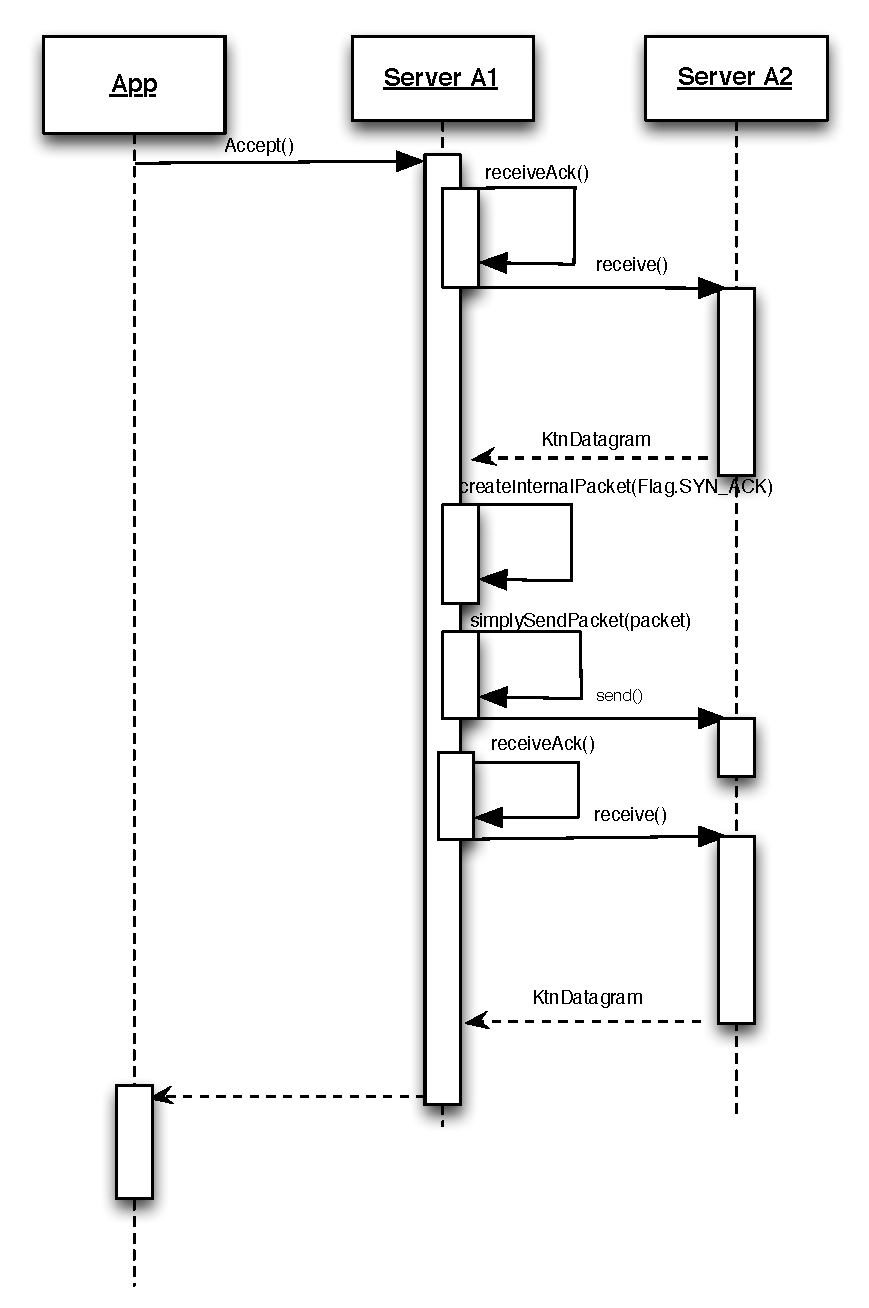
\includegraphics[scale=0.8]{ktnAccept.pdf}
\subsection{receive()}
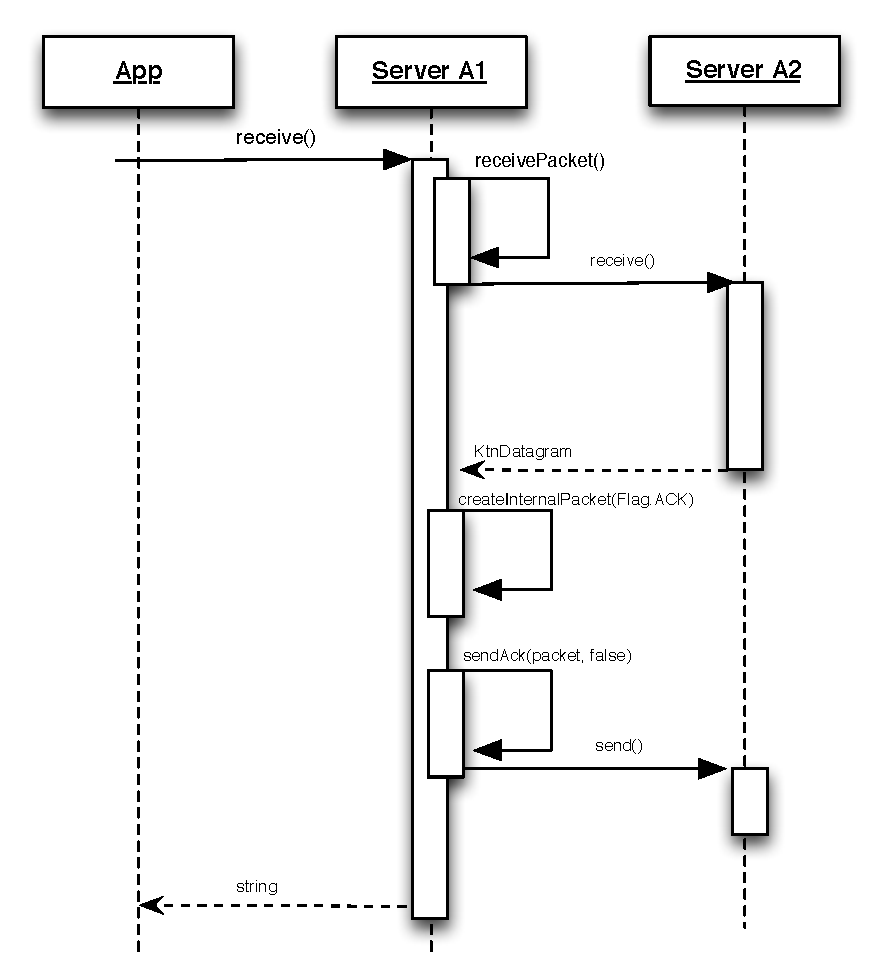
\includegraphics[scale=0.8]{ktnRecv.pdf}
\subsection{send()}
\includegraphics[scale=0.8]{ktnSend.pdf}
\newpage
\section{Disconnection}

For this discussion, lets presume that the clients initiate the close
operation using the \texttt{close()} method (Note: the server can also use the close
operation). This causes the client to send a \texttt{SYN} packet with the 
\texttt{FIN} bit set to 1, and enter the \texttt{FIN\_WAIT\_1}.
While in the \texttt{FIN\_WAIT\_1} state the client waits for an 
\texttt{ACK} packet. Upon receiving the \texttt{ACK} packet the client
switches to \texttt{FIN\_WAIT\_2} state.

In \texttt{FIN\_WAIT\_2} state the client is expecting a \texttt{FIN%
} packet from the server. As mentioned above, it's possible to receive the 
\texttt{FIN} packet directly. Anyway, when the \texttt{FIN} packet is
received, the client will respond with an \texttt{ACK} packet, and enter the
\texttt{\texttt{TIME\_WAIT}} state. This state allows the client to re-send the last final 
\texttt{ACK} packet in case its lost. After the waiting period, the client
formally closes the connection.

The server will receive the \texttt{FIN} packet, send an \texttt{ACK} packet
as a response, and enter the \texttt{CLOSE\_WAIT} state. While in the close wait
state, the server sends a \texttt{FIN} packet to the client, and enters the 
\texttt{LAST\_ACK} state. In this state the server wait for a \texttt{ACK}
packet from the client. When the packet is finally received, the connection
is finally closed.

Note: The server can also terminate a connection, thereby switching roles
with the client.

\subsection{\texttt{close()}}
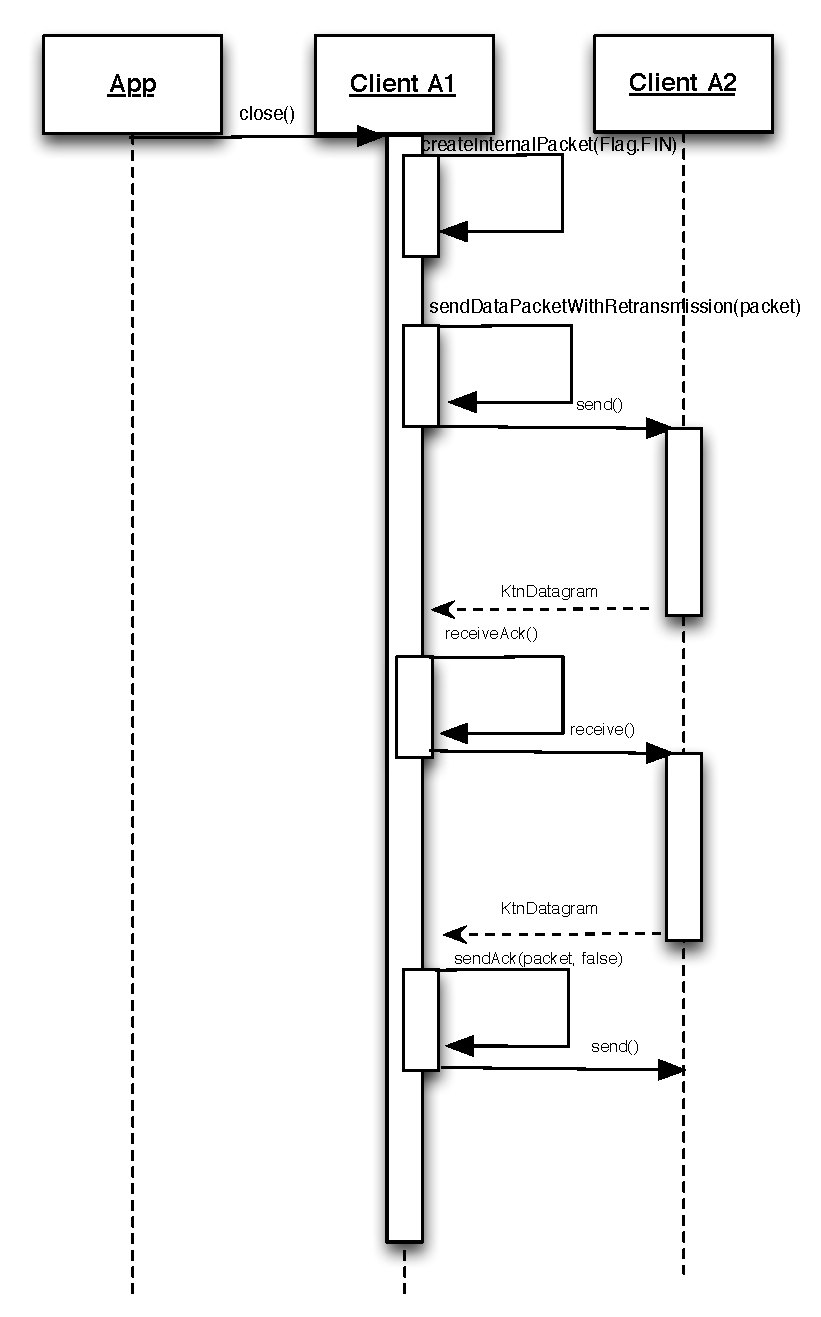
\includegraphics[scale=0.8]{ktnClientClose.pdf}
\subsection{ServerClose}
\includegraphics[scale=0.8]{ktnServerClose.pdf}

\subsection{ServerClose}

\section{Error Handling}

\subsection{Packet Loss}

When sending a packet the receiver of the packet will ask about it until the
packet is received. The packet is timed so that if the sender does not
receive an \texttt{ACK} during a given time(timeout), the sender will send
the packet again.

\subsection{Packet Delay}

A1 saves all the packets in a buffer, but it does not store duplicates. So
when the sender does not receive an \texttt{ACK}, it believes that the
packet is lost and sends it again. This means that the receiver gets two of
the same packet. This problem can be solved by checking the sequence number.
If a packet with the same sequence number has already been received, the
packet will be dropped, but the receiver will still send an \texttt{ACK} for
the duplicated packet.

\subsection{Packet Error/Corruption}

Right before a message is received it will be checked for errors using a
checksum to see if the packet contains any errors. If the packet does
contain errors an \texttt{ACK} will be sent, saying that the packet contains
errors.

\subsection{Ghost Packets}

The checksum will be checked and if it does not chek out be discarded. If it
is approved, the sequence number will be checked. If it does not have the
right sequence number it will be thrown away, if not it will be approved as
an ordinary packet.

\subsection{Packet Checks Out}

If the packet checks out it will be passed on upwards.

\end{document}
